\section{Layered Grid Architecture}
Following the work of Ian Foster, Carl Kesselman and Stevel Tuecke \cite{the_anatomy_of_the_grid}, the Grid Architecture identifies fundamental system components, and indicates how these components interact with one another. This Grid Architecture is first and foremost a protocol architecture, since the interoperability among any potential participant is the central issue and thus requires the definition of common protocols. Protocols govern the \textit{interaction} between components in the Grid and not the \textit{implementation}, maintaining local control.

\begin{quotation}
    \textit{"Why are protocols critical to interoperability? A protocol definition specifies how distributed system elements interact with one another to achieve a specified behavior and the structure of the information exchanged during this interaction. This focus on externals (interactions) rather than internals (software, resource characteristics) has important pragmatic benefits." \cite{the_anatomy_of_the_grid}}
\end{quotation}

In order to provide abstractions to interact with the Grid and develop applications that use it, application programming interfaces (APIs) and software development kits (SDKs) must also be provided; these are built on top of the protocols.
Together, APIs, SDKs and the protocols in the architecture constitutes a middleware.

The architecture is organized in a layer structure (\textit{figure \ref{fig:grid_protocol_architecture_and_internet_protocol_architecture}}), where components within each layer share common characteristics but can build on capabilities and behaviors provided by any lower level. The number of protocols must be contained, focusing on resource and connectivity protocols.

\begin{figure}[!ht]
    \centering
    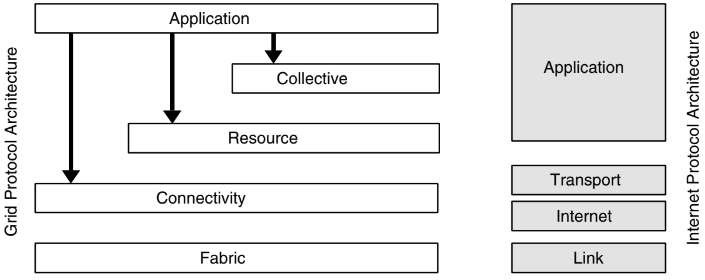
\includegraphics[scale=1]{document/chapters/chapter_2/images/grid_protocol_architecture_and_internet_protocol_architecture.png}
    \caption{Layered architecture relationship to Internet Protocol (IP) architecture. \cite{the_anatomy_of_the_grid}}
    \label{fig:grid_protocol_architecture_and_internet_protocol_architecture}
\end{figure}

\subsection{Fabric layer}
TODO

\subsection{Connectivity layer}
TODO

\subsection{Resource layer}
TODO

\subsection{Collective layer}
TODO

\subsection{Application layer}
TODO
